\chapter{Grundlagen}

Zunächst werden für ein besseres Verständnis der Arbeit die eingesetzten Materialien und Grundlagen vorgestellt. Zu diesen zählen diverse Hardware, wie das verwendete Smartphone, aber auch Software wie unter anderem die Entwicklungsumgebung oder das verwendete SDK (Software Development Kit) für die native Evaluationsanwendung. Zudem wird eine Einführung in die Begrifflichkeiten wie native und hybride Anwendungsentwicklung gegeben.

\section{Android} \label{AndroidPlattform}

Android \footcite{Android} ist ein Betriebssystem für mobile Geräte wie Smartphones oder Tablets, ursprünglich entwickelt von der Firma Android, Inc., welche 2005 von Google aufgekauft wurde \footcite{AndroidHistory}. Mobile Anwendungen für Android Systeme werden in der Programmiersprache Java geschrieben und anschließend in Androids eigenes Format DEX (Dalvik Executable Format) konvertiert \footcite{AndroidCookbook}. Die Android UI Guidelines \footcite{AndroidGuidelines} geben Richtlinien für das Design der Benutzeroberfläche von Android Anwendungen vor.
\\
\\
Des Weiteren sind für Android Anwendungen unter anderem noch folgende Grundbedingungen formuliert, an welche sich bei der Planung der Anwendung gehalten wurde: Die Anwendung sollte einfach zu installieren, zu entfernen und zu updaten sein. Sie sollte ansprechend sein und die Anforderungen elegant umsetzen um auch bei vielen Features leicht bedienbar zu bleiben. Wichtig ist, dass die Anwendung stabil, skalierbar, bedienbar ist und angemessen auf Benutzereingaben reagiert.\footcite{AndroidCookbook}

\section{iOS}

iOS ist das native Betriebssystem von Apple für alle mobilen Apple Geräte, wie zum Beispiel das iPhone, iPad oder iMacs . Mobile Anwendungen für iOS werden in einer Programmiersprache  namens Swift entwickelt. Apple stellt zum Entwickeln eine eigene IDE zur Verfügung: XCode. Zum Entwickeln von nativen iOS-Anwendungen wird immer ein Apple Computer benötigt\footcite{iOS}. 
\\
\\
Die Richtlinien für das Design grafischer Benutzeroberflächen sind in den 'iOS Human Interface Guidelines' definiert. Die drei primären Grundsätze dabei lauten: Klarheit, Fügsamkeit und Tiefe (Clarity, Deference and Depth)\footcite{iOSGUI}. 

\section{Entwicklungsumgebung}

Das Android SDK ist eine Entwicklungsumgebung für das Android Betriebssystem, welches sich an Entwickler zur Erstellung von Android-Anwendungen wendet und ist für Windows, Linux und Mac OS verfügbar. Es benötigt für viele Hauptfunktionen ein JDK (Java Development Kit) \footcite{AndroidSDK}. Das SDK beinhaltet einen Emulator, der es möglich macht die Anwendung auch ohne angeschlossenes Smartphone zu testen. Als IDE (Integrated Development Environment) wurde Android Studio genutzt, welches 2014 von Google veröffentlicht wurde und so Eclipse als primäre Entwicklungsumgebung für Android Anwendungen ablöste. Android Studio basiert auf der IntelliJ IDEA Community Edition von JetBrains. \footcite{AndroidOP} Es beinhaltet intuitive Tools, die die Erstellung einer grafischen Benutzeroberfläche nach den Android UI Guidelines \footcite{AndroidGuidelines} erleichtern. 

\section{Native Anwendungs-Entwicklung}

Eine native Anwendung ist eine Anwendung, die für eine spezifische Plattform entwickelt wurde und die Schnittstellen dieser Plattform direkt benutzt\footcite{Varianten}. Dadurch kann die Anwendung mit dem Betriebssystem und andere Software, welche auf dem Gerät installiert ist, interagieren. So kann die native Anwendung auch die gerätespezi-fische Hardware und Software, wie zum Beispiel das GPS oder Kameras verwenden\footcite{nativeApp1}. Ein weiterer Vorteil der nativen Anwendungen ist, dass sie die Ressourcen des Geräts durch die einheitliche Nutzung der Schnittstellen zur Hardware optimal nutzen kön-nen\footcite{nativeApp1}. Die plattformspezifischen Bibliotheken bieten zudem alle nötigen Elemente für den Aufbau einer der spezifischen Guidelines entsprechenden Benutzeroberfläche. Eine native Anwendung bringt das maximale  Ergebnis bezüglich Look-And-Feel und Performance\footcite{Varianten}.

\section{Hybride / Cross-Platform Entwicklung}

Eine hybride Anwendung ist prinzipiell wie eine Web Anwendung, nur mit einem leichtgewichtigen nativen Container, welcher es erlaubt, auf native plattformspezifische Funktionalitäten und Hardware zuzugreifen. Wie auch Web Anwendungen werden hybride Anwendungen oft in Skript-Sprachen wie JavaScript, HTML5 und CSS programmiert\footcite{Varianten}. Auf diese Weise entsteht Code, der gemeinsam auf allen Plattformen genutzt werden kann. Dies hat den Vorteil, dass nur eine Anwendung gewartet werden muss und nicht eine pro Plattform, für die die Anwendung herausgegeben werden soll. Als ein Nachteil wird allerdings die Performance genannt, welche unter Umständen, wie zum Beispiel einer erhöhten Nutzung von Hardware-Komponenten, deutlich schlechter als bei der nativen Variante sein soll\footcite{Varianten}. Nachfolgende Abbildung  \ref{fig:VariantenAppEntwicklung} beschreibt noch einmal bildhaft den Unterschied zwischen den drei Entwicklungsvarianten: Nativ, Hybrid und Web: 
\clearpage

\begin{figure}[h]
	\centering
	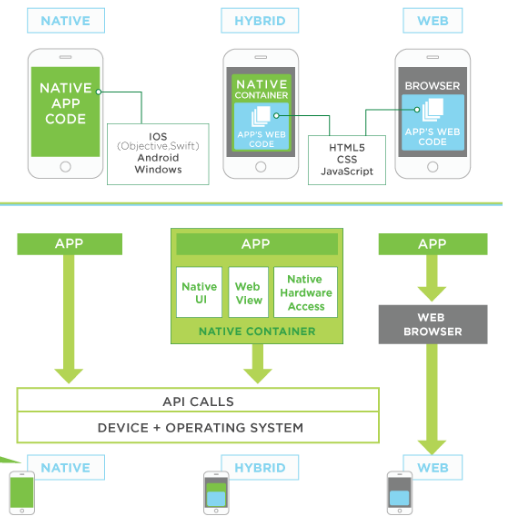
\includegraphics[width=0.5\textwidth]{Bilder/Vergleich_Nativ_Hybrid.PNG}
	\caption{Vergleich: native, hybride und Web Anwendungsentwicklung}
	\label{fig:VariantenAppEntwicklung}
\end{figure}

\section{Sensoren und andere Hardware in Smartphones}

Im folgenden wird die verwendete Hardware, sowie die gängigen Sensoren, welche in Smartphones eingebaut sind vorgestellt. Diese Sensoren werden in Anwendungen verwendet, um zum Beispiel die aktuelle Position zu bestimmen oder Feedback in Form von Vibrationen zu geben. 

\subsection{Das LG Nexus 5}

Für die Evaluation anhand einer zu entwickelnden Anwendung, welche unter anderem Hardware-Zugriffe auf Sensorik etc. testen soll, steht ein LG Nexus 5 als Gerät zur Verfügung. Das LG Nexus 5 erschien am 31. Oktober 2013 mit der Android-Version 4.4 KitKat. Es verfügt über ein Full HD IPS Display mit einer Bildschirmdiagonalen von 12,70 cm. Die Auflösung beträgt 1920 x 1080 Pixel. Das Smartphone besitzt eine 8 MP Kamera hinten und eine 1,3 MP Front-Kamera. Als Prozessor ist ein Qualcomm Snapdragon 800 mit einer Taktrate von 2,26GHz und 4 Kernen verbaut. Zudem ist das LG Nexus 5 mit folgenden Sensoren ausgestattet: Accelerometer, Gyroskop, Näherungssensor, Magnetometer und Barometer\footcite{Nexus5}. 

\subsection{Accelerometer und Gyroskop} \label{GrundlagenAccGyro}

Das Accelerometer, oder auch der Beschleunigungssensor, misst die Beschleunigung in X-, Y- und Z-Achsenrichtung. Unter Beschleunigung wird die Änderung der Geschwindigkeit zur Zeit verstanden. Im physikalischen Sinne ist jede Form von Änderung einer Bewegung, auch eine Abnahme der Geschwindigkeit oder Schwenken in eine andere Richtung, eine Beschleunigung. Das Gyroskop misst hingegen die rotatorische Geschwindigkeit, also Drehbewegungen. Zusammen mit dem Accelerometer erkennt das Smartphone so Bewegungsänderungen und kann darauf reagieren\footcite{AndroidWiki}. Die Ausrichtung der 3 Achsen von einem Smartphone ist in folgender Abbildung \ref{fig:Achsenausrichtung} dargestellt:

\begin{figure}[h]
	\centering
	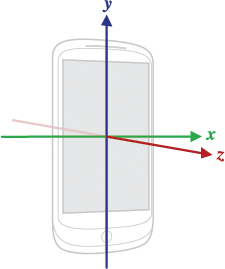
\includegraphics[width=0.5\textwidth]{Bilder/Axis_device.PNG}
	\caption{Schematisches Achsenmodell; Entnommen von: www.droidwiki.de/wiki/G-Sensor}
	\label{fig:Achsenausrichtung}
\end{figure}

\subsection{GPS}

GPS ist die Abkürzung für Global Positioning System und beschreibt ein System zur globalen Positionsbestimmung mit Hilfe von Satelliten. Smartphones mit GPS besitzen einen GPS-Chip, mit denen sie ihre Position auf 5-10 Meter genau bestimmen können\footcite{AndroidWiki}. Der GPS-Sensor ist relevant für zum Beispiel Navigations-Anwendungen. 

\subsection{Näherungssensor und Umgebungslichtsensor}

Der Näherungssensor bei Smartphones besteht üblicherweise aus einem Fotowiderstand und er dient zusammen mit dem Umgebungslichtsensor zur Messung der Helligkeit des Umgebungslichtes. Die Aufgabe des Näherungssensors ist es in der Regel, schnelle Änderungen der Umgebungshelligkeit festzustellen. Der Umgebungslichtsensor misst anhand des photoelektrischen Effekts das Umgebungslicht und passt daraufhin die beispielsweise automatisch die Display-Helligkeit an\footcite{AndroidWiki}. 

\subsection{Vibration}

Um auf Benutzereingaben eine Rückmeldung in Form eines Vibrationsfeedbacks zu geben, sind Vibrationsmotoren in Smartphones verbaut. Diese sind über die API des jeweiligen Betriebssystems ansprechbar. Gerade bei Geräten mit Touchscreen und ohne mechanische Tastatur kann ein solches Feedback es dem Benutzer vereinfachen, seine Eingabe als erfolgt zu erkennen\footcite{AndroidWiki}. 

\subsection{Magnetometer}

Ein  Magnetometer misst die magnetische Flussdichte und kann so bestimmen, wo sich der magnetische Norden befindet. Im Inneren des magnetometers befindet sich eine metallische Platte, welche unter Strom gesetzt wird. Durch das Wirken der Lorentzkraft auf diese Platte, deren Stärke abhängig von der Stärke des vorhandenen Magnetfeldes ist, wird diese verschoben. Das Magnetometer misst optisch oder elektrisch wie weit sich die Platte verschoben hat. Mit Hilfe des Magnetometers im Smartphone lassen sich Kompass-Anwendungen und Anzeigen der Blickrichtung auf Karten-Anwendungen realisieren\footcite{AndroidMag}. 